% preamble
\documentclass[11pt,reqno,oneside,a4paper]{article}
\usepackage[a4paper,includeheadfoot,left=25mm,right=25mm,top=00mm,bottom=20mm,headheight=20mm]{geometry}
%%%% DO NOT EDIT THIS FILE

% Standard packages
\usepackage{amssymb,amsmath,amsthm}
\usepackage{xcolor,graphicx}
\usepackage{verbatim}
\usepackage{mathtools}
\usepackage{hyperref}
% Layout of headers & footers
\usepackage{titling}
\usepackage{fancyhdr}
\newcommand{\runningtitle}{Running Title}
\pagestyle{fancy} \lhead{{\theauthor}} \chead{} \rhead{{\runningtitle}} \lfoot{} \cfoot{\thepage} \rfoot{}

% Hyphenation
\hyphenation{non-zero}

% Theorem definitions in the amsthm standard
\newtheorem{thm}{Theorem}
\newtheorem{lem}[thm]{Lemma}
\newtheorem{sublem}[thm]{Sublemma}
\newtheorem{prop}[thm]{Proposition}
\newtheorem{cor}[thm]{Corollary}
\newtheorem{conc}[thm]{Conclusion}
\newtheorem{conj}[thm]{Conjecture}
\theoremstyle{definition}
\newtheorem{defn}[thm]{Definition}
\newtheorem{cond}[thm]{Condition}
\newtheorem{asm}[thm]{Assumption}
\newtheorem{ntn}[thm]{Notation}
\newtheorem{prob}[thm]{Problem}
\theoremstyle{remark}
\newtheorem{rmk}[thm]{Remark}
\newtheorem{eg}[thm]{Example}
\newtheorem*{hint}{Hint}

%% Mathmode shortcuts
% Number sets
\newcommand{\NN}{\mathbb N}              % The set of naturals
\newcommand{\NNzero}{\NN_0}              % The set of naturals including zero
\newcommand{\NNone}{\NN}                 % The set of naturals excluding zero
\newcommand{\ZZ}{\mathbb Z}              % The set of integers
\newcommand{\QQ}{\mathbb Q}              % The set of rationals
\newcommand{\RR}{\mathbb R}              % The set of reals
\newcommand{\CC}{\mathbb C}              % The set of complex numbers
\newcommand{\KK}{\mathbb K}              % An arbitrary field
% Modern typesetting for the real and imaginary parts of a complex number
\renewcommand{\Re}{\operatorname*{Re}} \renewcommand{\Im}{\operatorname*{Im}}
% Upright d for derivatives
\newcommand{\D}{\ensuremath{\,\mathrm{d}}}
% Upright i for imaginary unit
\newcommand{\ri}{\ensuremath{\mathrm{i}}}
% Upright e for exponentials
\newcommand{\re}{\ensuremath{\mathrm{e}}}
% abbreviation for \lambda
\newcommand{\la}{\ensuremath{\lambda}}
% Make epsilons look more different from the element symbol
\renewcommand{\epsilon}{\varepsilon}
% Always use slanted forms of \leq, \geq
\renewcommand{\geq}{\geqslant}
\renewcommand{\leq}{\leqslant}
% Shorthand for "if and only if" symbol
\newcommand{\Iff}{\ensuremath{\Leftrightarrow}}
% Make bold symbols for vectors
\providecommand{\BVec}[1]{\mathbf{#1}}
% Hyperbolic functions
\providecommand{\sech}{\operatorname{sech}}
\providecommand{\csch}{\operatorname{csch}}
\providecommand{\ctnh}{\operatorname{ctnh}}
% sinc function
\providecommand{\sinc}{\operatorname{sinc}}
% closure of a set
\providecommand{\clos}{\operatorname{clos}}
% The absolute value of a real number or modulus of a complex number, with automatically scaling delimiters
\newcommand{\abs}[1]{\left\lvert#1\right\rvert}
\newcommand{\sgn}{\operatorname{sgn}}

% add two sub and superscripts with a space between them
\newcommand{\Mspacer}{\;} %Spacer for below Matrix display functions
\newcommand{\M}[3]{#1_{#2\Mspacer#3}} %Print a symbol with two subscripts eg a matrix entry
\newcommand{\Msup}[4]{#1_{#2\Mspacer#3}^{#4}} %Print a symbol with two subscripts and a superscript eg a matrix entry
\newcommand{\Msups}[5]{#1_{#2\Mspacer#3}^{#4\Mspacer#5}} %Print a symbol with two subscripts and two superscripts eg a matrix entry
\newcommand{\MAll}[7]{\prescript{#1}{#2}{#3}_{#4\Mspacer#5}^{#6\Mspacer#7}} %Print a symbol with two subscripts and two superscripts eg a matrix entry

% Make really wide hat for Fourier transforms applied to large functions
\usepackage{scalerel}
\usepackage{stackengine}
\stackMath
\newcommand\reallywidecheck[1]{%
\savestack{\tmpbox}{\stretchto{%
  \scaleto{%
    \scalerel*[\widthof{\ensuremath{#1}}]{\kern-.6pt\bigwedge\kern-.6pt}%
    {\rule[-\textheight/2]{1ex}{\textheight}}%WIDTH-LIMITED BIG WEDGE
  }{\textheight}%
}{0.5ex}}%
\stackon[1pt]{#1}{\scalebox{-1}{\tmpbox}}%
}
\providecommand{\widecheck}{\reallywidecheck}

\newcommand\reallywidehat[1]{%
\savestack{\tmpbox}{\stretchto{%
  \scaleto{%
    \scalerel*[\widthof{\ensuremath{#1}}]{\kern-.6pt\bigwedge\kern-.6pt}%
    {\rule[-\textheight/2]{1ex}{\textheight}}%WIDTH-LIMITED BIG WEDGE
  }{\textheight}%
}{0.5ex}}%
\stackon[1pt]{#1}{\tmpbox}%
}


%% Acknowledgements
\newcommand{\AckYNCSRP}[1]{#1 gratefully acknowledges support from Yale-NUS College summer research programme.}
\newcommand{\AckYNCProj}[1]{#1 gratefully acknowledges support from Yale-NUS College project B grant IG18-PRB102.}
\newcommand{\AckYNCWorkshop}[1]{#1 gratefully acknowledges support from Yale-NUS College workshop grant IG18-CW003.}
\newcommand{\AckNICA}[1]{#1 would like to thank the Isaac Newton Institute for Mathematical Sciences for support and hospitality during programme \emph{Complex analysis: techniques, applications and computations}, when work on this paper was undertaken. This work was supported by EPSRC Grant Number EP/R014604/1.}
\newcommand{\AckSMRIIVP}[1]{#1 would like to thank the Sydney Mathematics Research Institute for support and hospitality under the International Visitor Programme.}
 % Standard packages, page layout, theorem environments, macros, etc
% This file contains macros specific to the project.
% You are welcome to add your own macros, but please avoid deleting those written by others.

% Asymptotic notation
\newcommand{\bigoh}{\mathcal{O}}
\newcommand{\lindecayla}{\bigoh\left(\abs{\la}^{-1}\right)}
 % Macros specific to this project.
\author{Juwon Lee}
\title{Notes on Complex Analysis}
\renewcommand{\runningtitle}{Notes on Complex Analysis}
\date{\today}

\begin{document}
\maketitle
\thispagestyle{fancy}
%----------------------------------

\begin{abstract}
The goal of this document is to revise Complex Analysis relevant to the project. Thus, this document is not comprehensive on the subject. In addition, I aim to review my skills for LaTeX documentation. 
\end{abstract}

\section{Complex Numbers and Functions}

\subsection{Forms of Complex Numbers}
\begin{enumerate}
	\item \emph{Algebraic form}: $x + iy$ where $x,y \in \RR.$ 
	\item \emph{Geometric form}: $(x,y)$.
	\item \emph{Polar form}: $z =r(\cos\theta + i\sin\theta)$, where $$r = \sqrt{x^2+y^2} > 0, \cos \theta = \frac{x}{r}, \sin \theta = \frac{y}{r}.$$ 
The argument $z$ is not defined when $z=0$ or equivalently when $r=0.$
\end{enumerate}


% Textbook 1.4 Complex Functions
\subsection{Complex Functions}
We start by stating the definition of complex-valued function.

\begin{defn}{Complex-valued function.}
The complex-valued function $f$ of a complex variable is a relation that assigns to each complex number $z$ in a set $S$ a unique complex number $f(z).$ 
\end{defn}

\begin{defn}{Domain.}
The set $S$ is a subset of the complex numbers and is called the domain of definition of $f.$ 
\end{defn}

\subsection{Visualization}
Real-valued functions require two dimensions for visualization, the $x$-plane and the $y$-plane. 
Following this, the visualization of complex-valued functions requires four dimensions: two for variable $z$ and two for the values $w=f(z),$ as both $z$ and $w$ are comprised of real and imaginary parts. 
In reality, we use two planes, the $z$-plane and $w$-plane and view the function as a mapping from a subset of one plane to the other as shown in Figure 1.

\begin{figure}[htp]
	\centering
	% Be sure to save all figures inside the gfx directory or they will NOT be tracked by git
	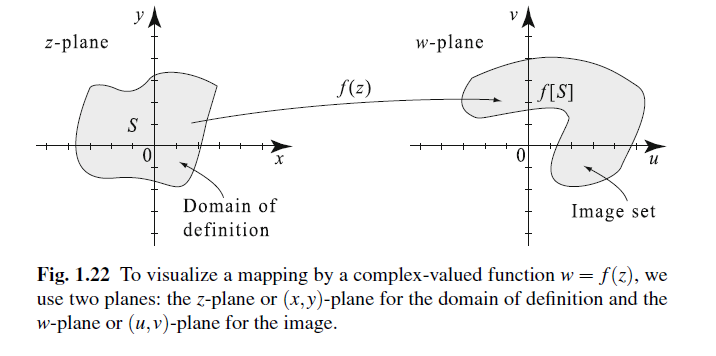
\includegraphics[width=0.8\linewidth]{gfx/complex function vis.png}
	\caption{Visualization for A Complex-valued Function}
	% \label{fig:complex function vis}
\end{figure}


\subsection{Linear Transformations}
Linear transformations can be thought of in terms of a dilation, a rotation, and a translation, which map regions to geometrically similar regions.




% Textbook 1.6 Complex Exponential
\subsection{Complex Exponentials}
For $x\in \RR,$ we recall that $$e^x = 1 + \frac{x}{1!} + \frac{x^2}{2!} + \frac{x^3}{3!} + \dots$$
Now, we extend the exponential function to the complex plane by substituting $x$ with a complex number $z$. 

\begin{defn}{Complex exponential function.}
For all $z \in \CC,$ 
$$e^z = \sum_{n=0}^{\infty} \frac{\abs{z}^n}{n!} =1+\frac{\abs{z}}{1!}+\frac{\abs{z}^2}{2!} + \dots < \infty .$$
\end{defn}

\begin{thm}{Euler's identity.} 
If $z=i\theta$ where $\theta \in \RR,$ then
$$e^{i\theta} = \cos \theta + i\sin\theta.$$
\end{thm}

\begin{cor}
For all $z = x+iy \in CC$ where $x, y \in \RR$, $$e^z = e^{x+iy} = e^xe^{iy} = e^x(\cos y + i\sin y).$$
This is the polar form of $e^z,$ where $\abs{e^z} = e^x$ and $\text{arg}(e^z) = y+2k\pi$ where $k\in\ZZ,$ visualized as the figure below.
\end{cor}

\begin{figure}
    \centering
    % Be sure to save all figures inside the gfx directory or they will NOT be tracked by git
    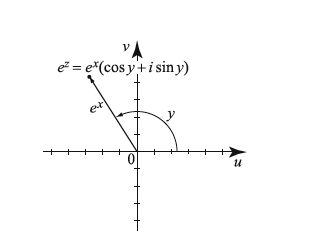
\includegraphics[width=0.8\linewidth]{gfx/complex exp vis.png}
    \caption{The modulus and argument of $e^z$}
    \label{fig:complex exp vis}
\end{figure}


Euler's identity function is proven using Definition 3 and the power series expansions for $\cos\theta$ and $\sin\theta.$ 
Since understanding the theorem is more important for this project than the proofs, I will not write the proof down. 
For better understanding of the theorem, I will solve the following example using Euler's identity.

\begin{eg}
$e^{2+i\pi} =  e^2(\cos\pi + i\sin\pi) =e^2(-1+0) = -e^2.$ 
From this polar form, we can find the argument and absolute of the complex exponential. For $k\in\ZZ,$
$$\abs{e^{2+i\pi}} = e^2, \text{arg}e^{2+i\pi} = \pi + 2k\pi.$$
\end{eg}

\begin{prop}{Exponential representation.}
Let $z = r(\cos\theta + i\sin\theta)$ with $r=\abs{z} > 0, \theta \in \RR, \text{arg}z = \theta+2k\pi.$ 
Then, $$z = re^{i\theta}.$$
\end{prop}




% Textbook 1.8 Logarithms and Powers
\subsection{Complex Logarithms}
The logarithm is defined as the inverse of the exponential function. 
For $z\in \CC \backslash {0},$ we define the complex function $w=\text{log} z$, therefore getting $$w=\text{log}z \Leftarrow \Rightarrow e^w = z.$$
To determine $w$ in terms of $z$, we write $w=u+iv$ and $z=re^{i\theta}$, with $\abs{z} = r > 0$ and $ \theta = \text{arg}z.$ 
Then, $$e^{u+iv} = e^ue^{iv} = z = re^{i\theta}$$ and hence $e^u = r $ and $e^{iv} = e^{i\theta}.$
This means that $u = \text{ln}r$, and $v$ and $\theta$ differ by an integer multiple of $2\pi$ because the complex exponential $2\pi i$ is periodic. 
So $v = \theta + 2k\pi \Rightarrow v = \text{arg}z$ where $k\in\ZZ.$

\begin{defn}{Complex logarithm.}
The formula for the complex logarithm is $$\text{log}z = \text{ln} \abs{z} + i\text{arg}z .$$
\end{defn}

\begin{eg}
We know that $\abs{i} = 1$ and $\text{arg}i = \frac{\pi}{2} + 2k\pi.$ From this, we can obtain $\text{log}i$ to be the following.
	\begin{align*}
	\text{log}i &= \text{ln}\abs{i} + i\text{arg}i\\
	&= \text{ln}1 + i(\frac{\pi}{2} + 2k\pi)\\
	&= i(\frac{\pi}{2} + 2k\pi)
	\end{align*}
\end{eg}

\begin{defn}{Principal branch.}
The principal value or branch of the complex logarithm is defined by 
$$\text{Log}z = \text{ln}\abs{z} + i\text{Arg}z.$$
$\text{Log}z$ is the particular value of log $z$ whose imaginary part is in the interval $(-\pi,\pi]$. 
\end{defn}

\begin{defn}{Branch.}
Let $\alpha$ be a fixed real number. For $z \neq 0,$ we call the unique value of arg$z$ that falls in the interval $(\alpha,\alpha+2\pi]$ the $\alpha$-th branch of arg $z$, denoting it by $\text{arg}_\alpha z.$
$$\text{log}_\alpha z = \text{ln}\abs{z} + i\text{arg}_\alpha z, \text{where}, \alpha < \text{arg}_\alpha z < \alpha+2\pi$$
\end{defn}

\subsection{Complex Powers}
\begin{defn}{Complex power.}
For $z \in \CC,$ $$z^a = e^{a\text{log}z}$$ where log$z$ is the complex logarithm. 
\end{defn}

\begin{eg}{Evaluating complex numbers}
	\begin{enumerate}
	\item Using the principal branch of the logarithm in Definition 6, we know that Log$(-i)$ = ln$\abs{-i} + \text{Arg}(-1) = 0+\frac{-i\pi}{2}.$ Using the Definition 8, we obtain
		\begin{align*}
		(-i)^{1+i} &= e^{(1+i)\text{Log}(-i)}\\
		&= e^{(1+i)\frac{-i\pi}{2}}\\
		&= e^{\frac{-i\pi}{2}+\frac{pi}{2}} = -ie^\frac{\pi}{2}
		\end{align*}
	\item Using the logarithm with a branch cut at angle $0$ in Definition 7, we obtain
		$$
		(i)^{1+i} = e^{(1+i)\text{log}_0(-i)} = e^{(1+i)\frac{3i\pi}{2}} = -ie^\frac{-3\pi}{2}.
		$$
	\end{enumerate}
\end{eg}




%----------------------------------


% Chapter 2 Analytic Functions
\section{Analytic Functions}

\subsection{History and Cauchy's Contributions}
Most of the theory of analytic functions is due to Augustin-Louis Cauchy.
\begin{enumerate}
	\item Defined the derivative and integral of complex functions
	\item Defined the notion of limit for functions and gave rigorous definitions of continuity and differentiability for real-valued functions
	\item Developed groundwork for the theory of definite integrals and series 
	\item Established theoretical aspects of complex analysis with great attention to rigorous mathematical proof which characterizes pure mathematics
\end{enumerate}

\subsection{Open Sets}
\begin{defn}{Neighborhoods.}
Let $r>0$ be a positive real number and $z_0$ a point in the plane. The $r$-neighborhood of $z_0$ is the set of all complex numbers $z$ satisfying $\abs{z-z_0} < r.$ We denote this set by $B_r(z_0).$
\end{defn}

\begin{defn}{Deleted Neighborhood.}
$$B'_r(z_0) = {z: 0 < \abs{z-z_0} < r}.$$
\end{defn}

\begin{defn}
Let $S$ be a subset of $\mathbb{C}$.  
\begin{enumerate}
	\item Interior point: $z_0$ is an interior point of $S$ if we can find a neighborhood of $z_0$ that is wholly contained in $S$.
	\item Boundary point: $z$ in the complex plane is called boundary point of $S$ if every neighborhood of $z$ contains at least one point in $S$ and at least one point not in $S$. 
	\item Boundary: the set of all boundary points of $S$ is called the boundary of $S$.
\end{enumerate}
\end{defn}

\begin{defn}{Closure.}
A subset $S$ of the complex numbers is called open if every point in $S$ is an interior point of $S$. An r-neighborhood, $B_r(z_0)$ is an open disk of radius $r$ centered at $z_0.$ Sets that contain all of their boundary points are called closed. For example, ${z: \abs{z-z_0} \leq r}$ is a closed disk. The smallest closed set that contains a set $A$ is called the closure of $A$.  
\end{defn}

\begin{defn}{Complex Derivative.}
Let $f$ be defined on an open subset $U$ of $\mathbb{C}$ and let $z_0 \in U.$ We say that $f$ has a complex derivative at the point $z_0$ if the limit $$\lim{z\to z_0}\frac{f(z)-f(z_0)}{z-z_0}$$ exists. This is called the complex derivative of $f$ at $z_0$ and is denoted by $f'(z_0)$.
\end{defn}
We say that $f$ is analytic on $U$ if it has a complex derivative at every point in $U$.

\begin{defn}{Entire function.}
An analytic function defined on the complex plane is said to be entire. 
\end{defn}

\begin{lem}
If $c$ is a constant, $f(z) = cz \Rightarrow f'(z) = c.$ 
\end{lem}

\begin{thm}
An analytic function defined on an open subset of the complex plane is continuous.
\end{thm}

\begin{lem}
Discontinuous function at $z_0$ does not have a complex derivative at $z_0.$
\end{lem}

\begin{thm}{Properties of Analytic Functions.}
Suppose that $f$ and $g$ are analytic functions on an open subset $U$ of the complex plane and let $c_1,c_2$ be complex constants. Then,
\begin{enumerate}
	\item $c_1f+c_2g$ and $fg$ are analytic on $U$ and for all $z \in U$.
	\item The function $fg$ is analytic on $U$ and for all $z \in U.$
	\item The function $\frac{f}{g}$ is analytic on $W = U \setminus {w\in U : g(w) = 0}$ and for all $z\in W$, 
	$$ (\frac{f}{g})'(z) = \frac{f'(z)g(z)-f(z)g'(z)}{(g(z))^2}$$
\end{enumerate}
\end{thm}

\begin{thm}{Cauchy-Riemann Equations}
Let $U$ be an open subset of $\mathbb{R}^2$ and let $u,v$ be real-valued functions defined on $U.$ Then the complex-valued function $f(x+iy) = u(x,y) + iv(x,y)$ is analytic on $U$ if and only if $u,v$ are differentiable functions on $U$ and satisfy $$u_x=v_y, u_y = -v_x$$ for all points in $U$. If this is the case, then for all $(x,y)\in U$, we have $$f'(x+iy) = u_x(x,y)+iv_x(x,y) \text{or} f'(x_iy) = v_y(x,y) - iu_y(x,y).$$
\end{thm}




\subsection{Differentiation of Functions of Exponential and Power Functions}

\begin{thm}{Derivative of the complex exponential function.}
Let $f(z) = e^z$ where $z\in\CC.$ Then $f$ is analytic on all of $\CC$ and $f'(z) = e^z.$
\end{thm}


\begin{thm}{Derivative of the complex logarithmic function.}
Let $f(z)=\text{Log}(z)$ where $\text{Log}(z)=\text{log}\abs{z}+i\text{Arg}(z)$ where Arg$(z)$ is such that $0< \text{Arg}(z)<2\pi$, i.e., the principal branch of the logarithmic function.
Then $f$ is analytic on all of $\CC \setminus \{x+yi \in \CC : x \geq 0, y = 0\}$, and $f'(z)=\frac{1}{z}$ on this set.
\end{thm}

% Chain rule and mean value theorems, p127
\begin{thm}{Chain rule.}
Let $u$ be a differentiable fnction on an open subset $W$ of $\RR^2$ and let $x,y$ be differentiable functions of $t$ defined on an open interval $I$ on the real line such that $(x(t),y(t))$ lies in $W$ for all $t \in I.$ 
Then $U(t) = u(x(t),y(t))$ is differentiable for all $t \in I$ and we have 
$$ frac{dU}{dt} = frac{\partial u}{\partial x} \frac{dx}{dt} + frac{\partial u}{\partial y} \frac{dy}{dt}.$$
\end{thm}





















\end{document}

